

%%% ----------------------------------------------------------------------
%%%%%%%%%%%%%%%%%%%%%%%%%%%%%%%%%%%%%%%%%%%%%%%%%%%%%%%%%%%%%%%%%%%%%%%%%%

\chapter{Basic Examples}

There is a deep part of the author that does not want to begin with these examples.  There is a real danger for the cursory observer to see these and hastily conclude that our work, or \proglang{R} as a whole, is merely a ``Matlab Clone.''  Nothing could be further from reality.

Matlab is an amazing product.  It costs quite a lot of money; it had better damn well be.  However, for statistics, machine learning, data mining --- data science --- we believe that \proglang{R} is ``better.''  Is \proglang{R} faster?  Emphatically, no.  But we argue that \proglang{R} wins in other ways.

It is true that everything \proglang{R} can do, so too can Matlab; of course, the converse is also true --- that everything Matlab can do, \proglang{R} can do as well.  Each is a turing complete language.  But being turing complete is not sufficient; \LaTeX\ is turing complete, and yet we do not perform scientific computation in it (although of course it is unparalleled in typesetting).  But we could.  

The fact that we do not is an extension of the fact that math journals do not publish articles written in \proglang{C} or \proglang{Fortran}.  Those programming languages are the wrong mediums of abstraction for expressing highly complicated ideas to domain experts.  Only a madman would attempt to express deep mathematical abstraction in these languages for publication (implementation being an entirely separate issue).  Likewise, we do not perform our statistical analyses in \LaTeX\ (don't be a pedant; we are not talking about sweave and you know it).  People overwhelmingly choose \proglang{R} for the analysis of data because it is the closest brain~$\rightarrow$~computer translation available for such problems.

Of course, this goes both ways.  If your life is matrix algebra, then \proglang{R} is a much worse fit for you than is Matlab.  Much of statistics is applied matrix algebra, but not all matrix algebra is statistics.

So we reluctantly press on with several basic examples utilizing distributed matrices.  For meatier examples, see Chapter~\ref{chpt:avdstat}.




\section{Reductions and Transformations}

\subsection{Reductions}

In Section~\ref{sub:diag}, we discussed the way that the \code{diag()} method may be utilized as a reduction operator.  We have numerous other reductions available, such as \code{sum()}, \code{prod()}, \code{min()}, and \code{max()}.  These operate exactly as their serial counterparts:
\begin{lstlisting}[language=rr,title=Reductions]
library(pbdDMAT, quiet = TRUE)
init.grid()

dx <- ddmatrix(data=0:1, nrow=10, ncol=10)

sm <- sum(dx)
comm.print(sm)

pd <- prod(dx)
comm.print(pd)

mn <- min(dx)
comm.print(mn)

mx <- max(dx)
comm.print(mx)

finalize()
\end{lstlisting}

We also offer some ``super reductions''.  It is possible to change a distributed matrix into a non-distributed matrix or vector using the methods \code{as.matrix()} or \code{as.vector()}.  For example:

\begin{lstlisting}[language=rr,title=Super Reductions]
library(pbdDMAT, quiet = TRUE)
init.grid()

dx <- ddmatrix(data=0:1, nrow=10, ncol=10)
print(dx)

x <- as.matrix(dx)
comm.print(x)

finalize()
\end{lstlisting}

These can be very useful in testing, but should be used sparingly at scale.




\subsection{Transformations}

We also offer numerous in-place transformations, such as the various \code{log()} functions, \code{abs()}, \code{sqrt()}, \code{ceiling()}, \code{floor()}, and \code{round()}.  For example:

\begin{lstlisting}[language=rr,title=Transformations]
library(pbdDMAT, quiet = TRUE)
init.grid()

comm.set.seed(diff = TRUE)

dx <- ddmatrix(data=-3:3, nrow=10, ncol=10)

dx <- ceiling(sqrt(abs(dx)))

x <- as.matrix(dx)
comm.print(x)

finalize()
\end{lstlisting}





\section{Matrix Arithmetic}

We also offer a complete set of methods for distributed matrix arithmetic.  With identical syntax to \proglang{R}, we can do some reasonably complicated things, such as:

\begin{lstlisting}[language=rr,title=Transformations]
library(pbdDMAT, quiet = TRUE)
init.grid()

dx <- ddmatrix(data=-3:3, nrow=10, ncol=10)
vec <- 1:2

dy <- (dx - vec) %*% dx

y <- as.matrix(dy)
comm.print(y)

finalize()
\end{lstlisting}

For a full list of methods, see the \pkg{pbdDMAT} documentation.


One item worth noting is that, as with regular \proglang{R}, if the user wishes to compute $X^TX$ or $XX^T$, then it is usually much faster to use the methods \code{crossprod()} and \code{tcrossprod()}, respectively.  However, for this operation, things are somewhat more complicated in the distributed sphere than in serial.  
\begin{figure}[ht]
\centering
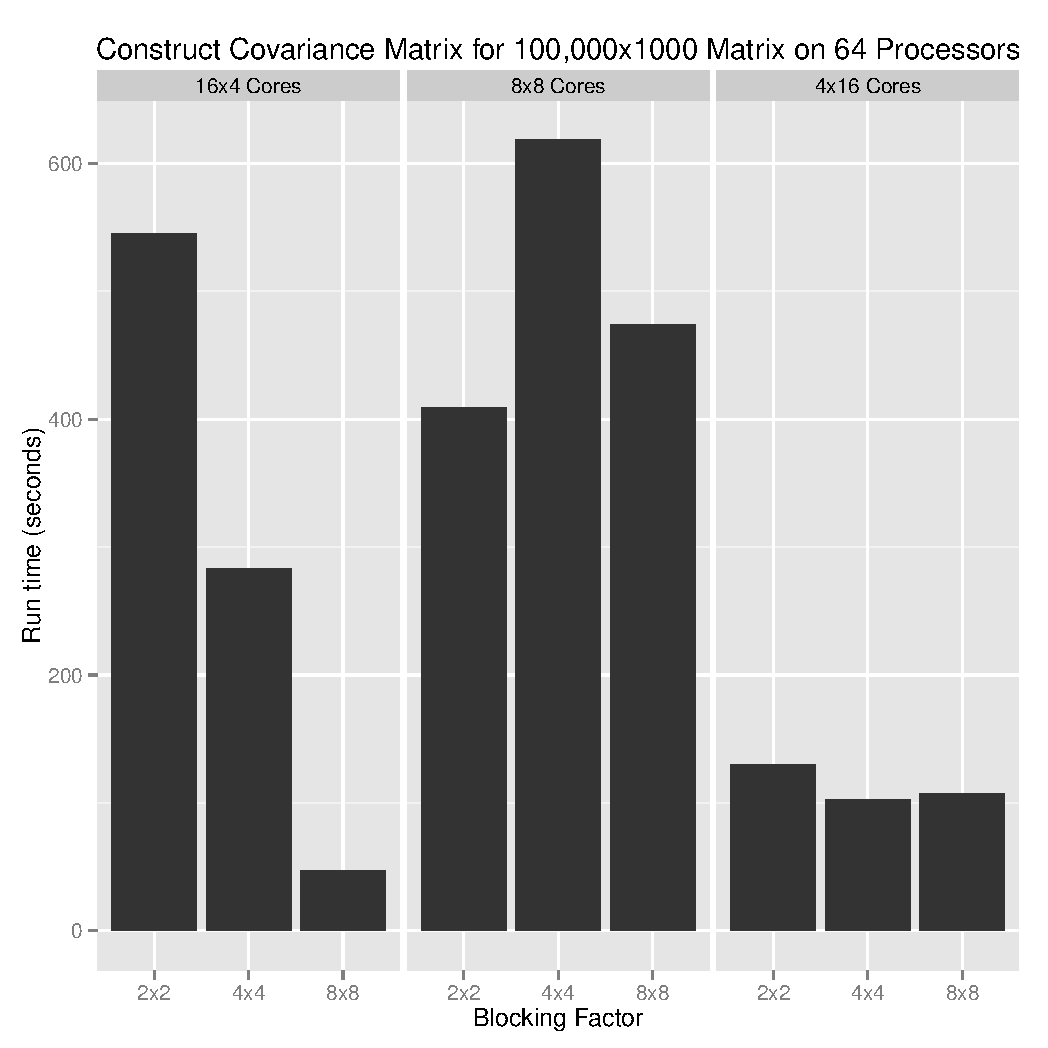
\includegraphics[scale=.6]{pbdDEMO-include/pics/cov.pdf}
\caption[Covariance Benchmark]{Covariance Benchmark Showing Effect of Parameter Calibration}\label{fig:cov}
\end{figure}
Figure~\ref{fig:cov} shows the results of a benchmark of the \code{cov()} method for computing variance-covariance matrices (which is just a small amount of extra work on top of \code{crossprod()}).  Here, each run consists of 25 replicates of calling \code{cov()} (which calls \code{crossprod()}) and then reporting the average run time.  The changes in parameters are subtle, but the effects are enormous.  Sometimes is may be (much) more beneficial to use \code{t(x) \%*\% x}.  Others it may not.  Proper calibration of these parameters to achieve optimal performance for a given task is still somewhat of an open question to the HPC community.





\section{Matrix Factorizations}

In addition to all of the above, we also provide several of the more important matrix factorizations for distributed matrices.  Namely, the singular value decomposition
\code{svd()}/\code{La.svd()},~\index{Code!\code{svd()}}\index{Code!\code{La.svd()}}
QR factorization \code{qr()},~\index{Code!\code{qr()}}
Cholesky factorization \code{chol()},~\index{Decomposition!Cholesky}\index{Code!\code{chol()}}
and LU factorization \code{lu()}.~\index{Decomposition!LU}\index{Code!\code{lu()}}
So for example:

\begin{lstlisting}[language=rr,title=Matrix Factorizations]
library(pbdDEMO, quiet = TRUE)
init.grid()

comm.set.seed(diff = TRUE)

dx <- ddmatrix("rnorm", nrow=10, ncol=10, bldim=2)

out <- chol(crossprod(dx))
print(out)

finalize()
\end{lstlisting}




\section{Exercises}
\label{sec:basic_example_exercise}

\begin{enumerate}[label=\thechapter-\arabic*]

\item
Sub-setting, selection and filtering are basic matrix operation featured
in \proglang{R}. The next may look silly, but it is useful for data
processing.
Suppose $\bX$ is in \code{ddmatrix} with dimension $97\times 42$,
say \code{dX <- ddmatrix(rnorm(97 * 42), nrow=37)}, do the following:
\begin{itemize}
\item
  \code{dY <- dX[c(1, 41, 5, 4, 3),]} \\
  \code{dY <- dX[, c(10:3, 5, 5)]} \\
  \code{dY <- dX[3:51, 5:3]}

\item
  \code{dY <- dX[dX[, 31] > 10,]} \\
  \code{dY <- dX[dX[, 41] > dx[, 40],]} \\
  \code{dY <- dX[, dX[41,] > dx[40,]]} \\
  \code{dY <- dX[dX[, 41] > dx[, 40], c(1, 3, 5)]}

\item
  \code{dX[c(1, 41, 5, 4, 3),] <- 10} \\
  \code{dX[, c(10:3, 5, 5)] <- 9} \\
  \code{dX[3:51, 5:3] <- 8}

\item
  \code{dX[dX[, 31] > 0,] <- 7} \\
  \code{dX[dX[, 41] > dx[, 40],] <- 6} \\
  \code{dX[, dX[41,] > dx[40,]] <- 5} \\
  \code{dX[dX[, 41] > dx[, 40], c(1, 3, 5)] <- 4}

\item
  \code{dX[c(1, 40, 5, 4, 3),] <- dX[c(1, 41, 5, 4, 3) + 1,]} \\
  \code{dX[, c(10:3, 5, 5)] <- dX[, c(10:3, 5, 5) + 1]} \\
  \code{dX[c(10:3, 5, 5),] <- dX[c(10:3, 5, 5) + 1,]} \\
  \code{dX[3:51, 5:3] <- dX[(3:51) + 1, (5:3) + 1]}

\item
  \code{dX[dX[, 31] > 0,] <- dX[dX[, 31] > 0, c(42, 1:41)]} \\
  \code{dX[dX[, 41] > dx[, 40],] <- dX[dX[, 41] > dx[, 40], c(41:42, 1:40)]} \\
  \code{dX[, dX[41,] > dx[40,]] <- dX[c(96:97, 1:95), dX[, 41] > dx[, 40]]} \\
  \code{dX[dX[, 41] > dx[, 40], c(1, 3, 5)] <- dX[dX[, 41] > dx[, 40], c(1, 3, 5) + 1]}
\end{itemize}
If any of above does not work, please report the bugs.
\label{ex:basic1}


\item
Suppose \code{dX} is as Exercise~\ref{ex:basic1}, do the following:
\begin{itemize}
\item
  \code{dY <- dX[-c(1, 41, 5, 4, 3),]} \\
  \code{dY <- dX[, -c(10:3, 5, 5)]} \\
  \code{dY <- dX[-(3:51), -(5:3)]}

\item
  \code{dY <- dX[dX[, 41] > dx[, 40], -c(1, 3, 5)]}

\item
  \code{dX[-c(1, 41, 5, 4, 3),] <- 10} \\
  \code{dX[, -c(10:3, 5, 5)] <- 9} \\
  \code{dX[-(3:51), -(5:3)] <- 8}

\item
  \code{dX[dX[, 41] > dx[, 40], -c(1, 3, 5)] <- 4}

\item
  \code{dX[-c(1, 40, 5, 4, 3),] <- dX[-(c(1, 41, 5, 4, 3) + 1),]} \\
  \code{dX[, -c(10:3, 5, 5)] <- dX[, -(c(10:3, 5, 5) + 1)]} \\
  \code{dX[-c(10:3, 5, 5),] <- dX[-(c(10:3, 5, 5) + 1),]} \\
  \code{dX[-(3:51), -(5:3)] <- dX[-((3:51) + 1), -((5:3) + 1)]}

\item
  \code{dX[dX[, 41] > dx[, 40], -c(1, 3, 5)] <- dX[dX[, 41] > dx[, 40], -(c(1, 3, 5) + 1)]}
\end{itemize}
% If any of above does not work, please report the bugs.
\label{ex:basic2}


\item
Verify the validity of Exercises~\ref{ex:basic1} and~\ref{ex:basic2} using 
ordinary \proglang{R} operations (cast the matrix as global first using 
\code{X <- as.matrix(dX)}).


\item
Implement SPMD row-major matrix format in 2 processors for 
Exercises~\ref{ex:basic1} and~\ref{ex:basic2}.


\end{enumerate}

